\documentclass{article}
\usepackage[margin=1.25in]{geometry}
\usepackage{amsmath, amssymb, setspace, enumerate, enumitem}
\usepackage{setspace}
\usepackage{graphicx}
\onehalfspacing

\begin{document}
    \begin{enumerate}
        \item \begin{enumerate}[label=(\alph*)]
            \item Two items will have high cosine similarity if they are pointing in roughly the same direction $\approx 1$, and they will have high Euclidean distance similarity if their points are far from each other.\\[0.25in]
            Two vectors parallel to each other, pointing at the same direction, and are close to each other, will have high cosine similarity and low Euclidean distance similarity.\\[0.25in]
            Two vectors parallel to each other, pointing in the opposite direction, and are far from each other, will have low cosine similarity and high Euclidean distance similarity.
            \item Cosine similarity will change because if the origin changes, the angles will change as well. Euclidean distance similarity will remain the same as the distance between two vectors will not change when the origin is changed.
        \end{enumerate}

        \item Consider the two cases present:\\
        $\pi \geq \frac{1}{2}$, then $e(f(x)) = 1 - \pi(x)$, $\pi(x) \geq 1 - \pi(x)$ based on our condition.\\
        $\pi < \frac{1}{2}$, then $e(f(x)) = \pi(x)$, $\pi(x) < 1 - \pi(x)$ based on our condition.\\
        Then, it appears that $e(f(x)) = min\{\pi(x), 1 - \pi(x)\}$ depending on the value of $pi$, which is either $\geq \frac{1}{2}$ or $< \frac{1}{2}$.\\[0.25in]
        $f(x)$ is our target function, so there is no other hypothesis that has a smaller error other than the target function, we build our hypothesis to attempt to guess the target hypothesis.

        \item \begin{enumerate}[label=(\alph*)]
            \item The decision boundary for 1-NN, blue represents +1, red represents -1: \\ 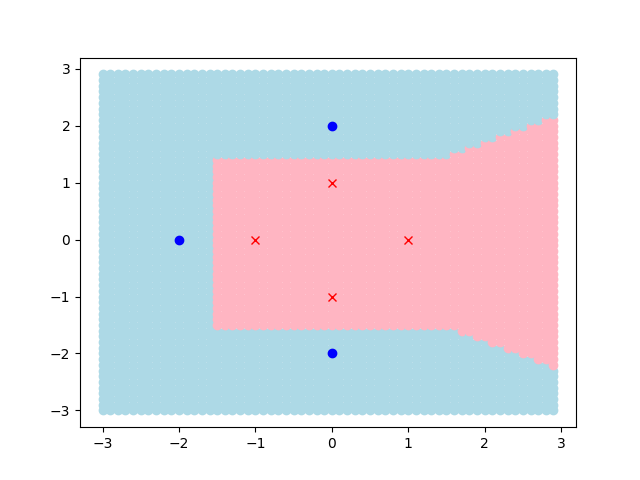
\includegraphics[scale=0.5]{images/p6_1_a.png}\\[0.25in]
            The decision boundary for 3-NN, blue represents +1, red represents -1: \\ 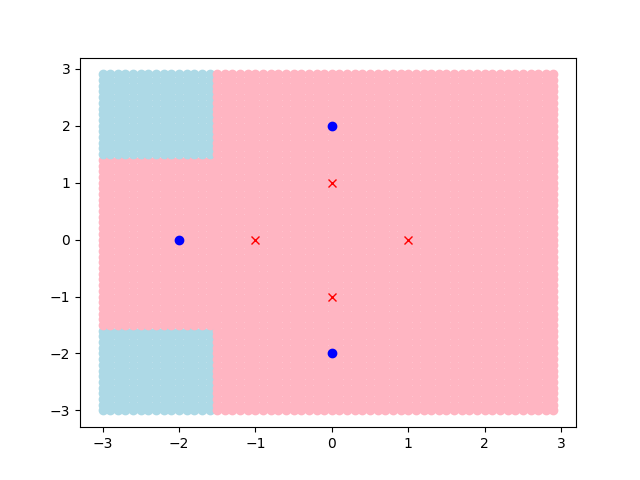
\includegraphics[scale=0.5]{images/p6_1_a_3.png}
            \item Decision boundaries are the same as previously mentioned, for 1-NN of the transformed dataset, we have \\ 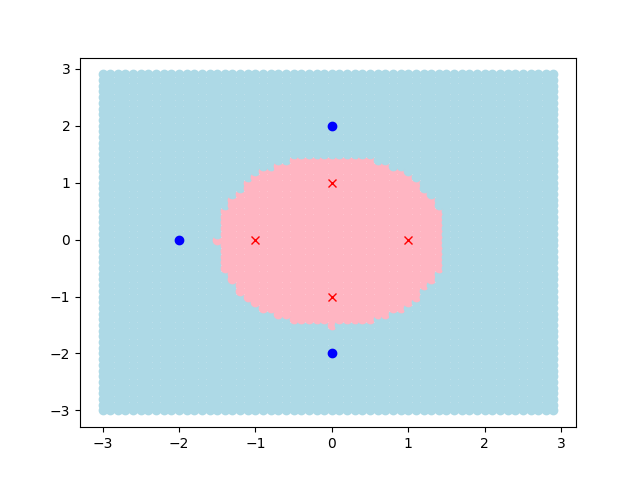
\includegraphics[scale=0.5]{images/p6_1_b.png}\\[0.25in]
            for 3-NN, we have \\ 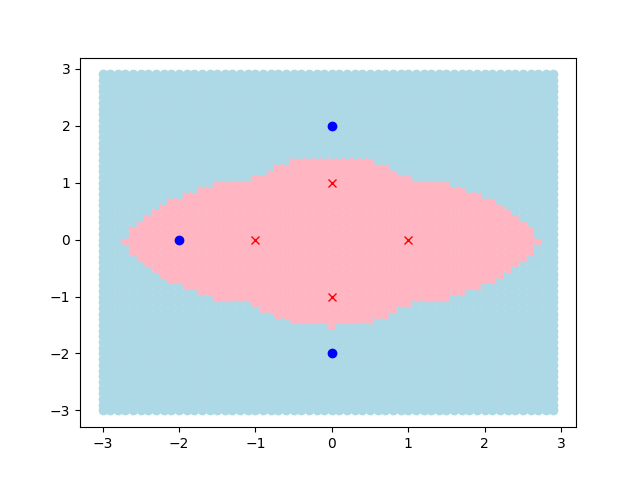
\includegraphics[scale=0.5]{images/p6_1_b_3.png}
        \end{enumerate}
        
        \item third
    \end{enumerate}
\end{document}